\chapter{Results and Discussion}

\section{Piezo1 as integrator of biomechanical events in MSCs}

\myworries{How does the peak relate to flow rate? Is there saturation?}
It is well known, that stem cell migration, differentiation and self-renewal is significantly influenced by physical interaction between the cell and the surrounding physical microenvironment. [Eyckmans2011][Lee2011] MSCs are arguably the most thoroughly studied type of stem cell in the context of mechanobiology, possibly because of relative ease of access and the promising potential they hold for regenerative medicine. Extensive studies of different properties of forces (e.g. nature, amplitude, oscillation) on MSCs give great insight into the reach of this underappreciated contribution to cell guidance. However, the significance of \Piezo{} and the associated calcium-ion influx in MSC mechanosensing is not fully understood. In the following part we want to elucidate whether \Piezo{} is functionally able to elicit a significant intracellular signal in MSCs.\\
In a reductionist approach, we conclude a significant contribution of \Piezo{} given MSCs exhibit a \Piezo{}-mediated influx of extracellular calcium ions in response to force. \\
For our first experiment, Flowchambers were prepared with wild-type (WT) cells being seeded and stained as described in \myworries{PUT REFERENCE}. For each flowchamber two calcium imaging recordings were carried out in close temporal sequence to each other: First recording was done using the previously mentioned flow rate protocol executed with modified, calcium-free ACSF as flow shear medium. Upon completion of the first recording, the flow shear medium is exchanged for normal, calcium containing ACSF and the cells flushed for 12 minutes with a flow rate of 0.2ml/min. After the 12 minute flushing period has ended, a second recording was done with the previously used flow rate protocol. After both measurements were completed, the integrity of the flowchamber was assessed by eye and the measurement deemed qualified for analysis, when no violation of structural integrity was observed. The sequence of first calcium-free and second calcium-containing medium is important, as reactive capability of the cells has to be demonstrated in the last measurement to rule out cell death as a possible explanation for lack of impulse response. We then processed the d

\begin{itemize}

    \item Increase of up to 80\% in fluorescence levels in pulse response. Significant difference in impulse response

    \item Two phenomena: Small negative bump (decrease in fluorescence) in pulse response and discontinuous jump between measurements.
    \item Bump: Fluorescent particles, non-adherent. When pulse, swept away, rigid segmentation only sees drop of fluorescence. The nature of those particles could either be exogenous particle with inherent properties that lead to higher measured fluorescence levels or there is a correlation between high intracellular calcium-ion level cells and adherence. Since effect size too small we did not investigate further.
    \item Missing calcium-signal after application of shear stimulus, if no external calcium-ions are supplied. 
    \item shows complete lack of calcium-influx response after shear stimulus with calcium-free medium as opposed by calcium-containing response. 
    \item Discontinuity: Possibly cells overcompensating the intracellular Calcium-stores when provided extracellular Calcium.
    \item Continuously decreasing fluorescence: Photobleaching! Keep in mind that second signal is likely higher.
    
\end{itemize}

\begin{figure}
    \centering
    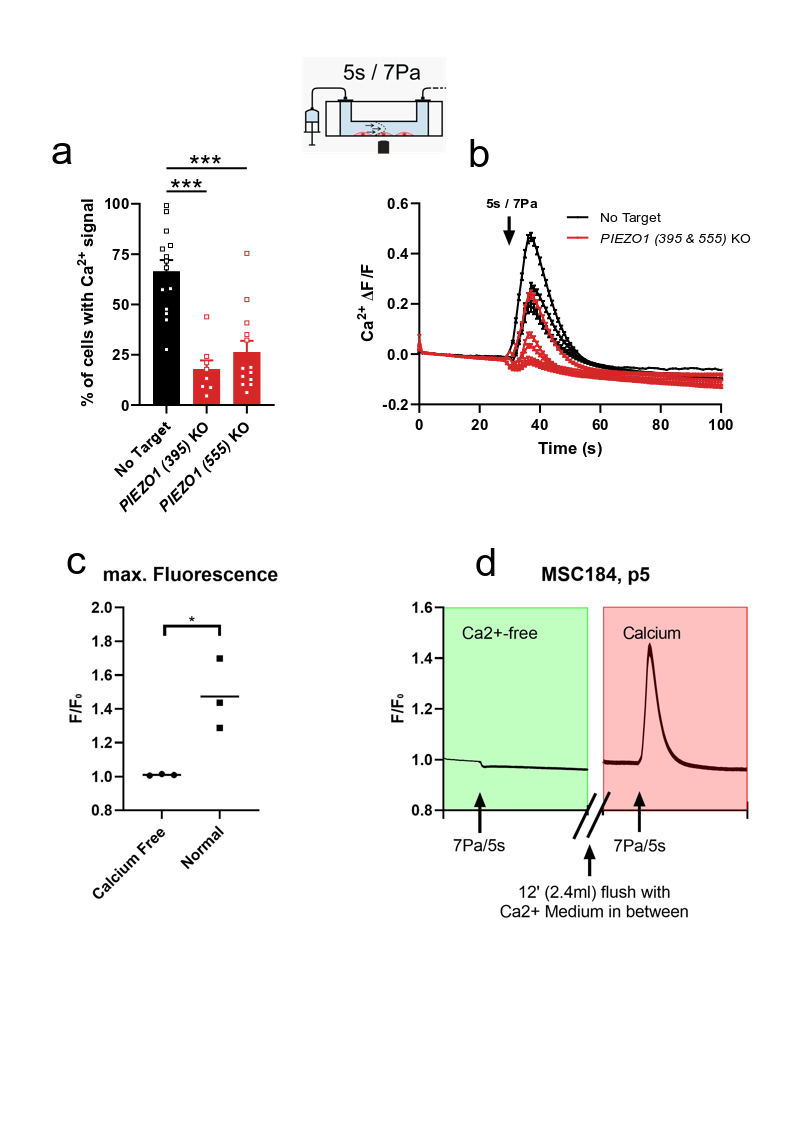
\includegraphics[width = 0.7\textwidth]{Combined_CalciumFree_KnockOut.png}
    \caption{Piezo1-mediated influx of extracellular Ca2+ confirmed as mechanotransductory event in MSC. \myworries{NEW ARRANGEMENT: D, C, B, A} \textit{Top:} Schematic drawing of Flowchamber. a.) Calcium-influx in response to fluidic shear pulse of 5s with an amplitude of 7Pa (Data points describe technical replicates, ***p$<$0.0001, ANOVA with Dunnette's multiple comparison test) b.) Same data as in previous graph with time-curve plotted c.) Peak values of fluorescence levels of samples in calcium-free and calcium-containing medium. (n = 3, *p $<$ 0.05, Student's t-test) d.) Representative donor measurement of medium comparison (Data contains pooled data of 4 technical replicates and is mean $\pm$ SEM)}
    \label{fig:Calcium}
\end{figure}

We demonstrated that MSCs exhibit reactive mechanosensitive capabilities through force-mediated rapid onset influx of extracellular Calcium-ions. The role of \Piezo{} in this process, however, is not defined. To shed light on the contribution size of \Piezo{} we compared the impulse response capabilities of two distinct \Piezo{}-knock out constructs to a control cell line.\\
In preparation for this experiment three transfected cell lines were generated (2 distinct \Piezo{} knock-out's and one negative control) using pre-made lentivirus, carrying a CRISPR/Cas9-system with puromycin resistance as the selection marker. The grouping is specified through the Lentiviral Construct used, resulting in cell line P1-395 (Deletion at \myworries{Ask MATTHIAS}), P1-555 and NoT (No Target, Control for the viral treatment with no putative genome mutation).  In order to assess knock-out efficiency, both Western Blot and qRT-PCR were done not more than one passage after thawing, to avoid overestimation of knock-out efficiency as it likely increases with growing passages. With an knockout efficiency on mRNA-level of XX\% in P1-395 and XX\% in P1-555 and a corresponding knockout-efficiency on protein-level of XX\% in P1-395 and XX\% in P1-555, respectively, we can consider this cell line a valid knock-out model. \myworries{Add efficiency numbers of knockout} 

We then seeded cells in flowchambers and measured the intracellular calcium signal of the cells in response to a shear pulse, similar to the protocol from the previous experiment but only with a single measurement per flowchamber with normal ACSF as shear flow medium. Intriguingly, the knock-out cells show a significantly reduced reaction capability when compared to control. \myworries{FigReference} When comparing the relative amount of cells that exhibit calcium-influx in response to shear stress, we see a 66\% decrease when comparing knock-out cells with control, with the effect being bigger in P1-395 (-73\%) as in P1-555 (-60\%). Interestingly, this difference between two different constructs regarding  their reduction of impulse response correlates well with the knock-out efficiency. Figure 3.b, which shows the same data, but over full temporal resolution illustrates how the area under the curve is largely reduced when \Piezo{} is knocked out. Modelling of the channel dynamics using a simple statistical model shows that, the decay mechanics largely stay the same with only the amplitude changing to lead to this result, or differently put: The model suggests that there is no compensating adaptation of single channel mechanics in response to lower channel abundance.

\myworries{WHY CHANGES OF METRICS? Cells that show Calcium Signal vs Max Fluorescence... Homogenize?}

These results confirm that \Piezo{} is the main driver in force-mediated calcium-influx in mesenchymal stem cells.


\section{Piezo1 and the extracellular matrix}

Preliminary mass spectroscopy secretome analysis of \Yoda-treated cells showed a distinct decrease in core extracellular matrix (ECM) components, such as alpha-1 type I collagen (\colone), Fibronectin-1 (\textsc{Fn1}) and finally alpha-1 type III collagen (\colthree) (Not shown here).
This inspired further investigation into this matter.\par

After seeding cells in serum-free medium and letting them rest, we chemically stimulated \Piezo{} with \Yoda{} during 30 minutes, before washing them and transferring them in the incubator again, following the protocol described earlier \myworries{REF}. We then harvested identical samples right after intervention (d0) and after 24, 48 and 72 hours (denoted d1, d2 and d3, respectively) to achieve temporal resolution. Western Blot of intracellular protein showed a distinct decline in \colone in samples that have been treated with \Yoda{}. \myworries{FigureRef} Furthermore, the effects were not only marked by fast onset but also of long-lasting nature, since the effect of a singular 30 minutes \Yoda{}-exposition remained the same three days after intervention.\par
We also looked at mRNA representation of identical samples through qRT-PCR, with investigated mRNA's including \colone{}, \colthree{}, \textsc{Fn}1 and Interleukin-6 (IL-6) with GAPDH and RPL13A as house-keeping genes to confirm our prior results.  All measurements were normalised against negative control samples harvested immediately after the intervention.\\
While we were not able to produce a significant result in any time point or gene, we saw a d


we saw a tendency of relative decrease in \colone{} over three days when comparing Piezo1-activation group with negative control group. Quite remarkably, the rapid downregulation of Protein in day 1 is not mirrored in RNA concentration, suggesting that the decrease in protein is the result of proteolytic activity. This divergence introduces a new dimension, inspiring further research into the topic.

While the results were surprising, follow-up studies are required before we can make any sound conclusions. We have good reasons as to think why increased secretion or reduced gene expression would likely not be a valid explanation for the observed reduction in \colone{} content. Neither RNA analysis suggests a decrease in gene transcription, nor does protein mass spectroscopy analysis of \Yoda{}-treated cells hint towards an increase in protein secretion. However, there is at least one alternative hypothesis. Maybe this data can be explained by a \Piezo{}-mediated protein degradation mechanism. For example, an abundantly expressed cytosolic protease that relies on an ionic cofactor (e.g. Calcium) for effector-function would be straightforward explanation. The protease family calpain suits this description. [Goll2003] Calpains are calcium dependent intracellular proteases with relatively high specificity and are considered rather regulatory than digestive proteases. The interaction between calpains and \colone has also already been observed, as Nassar and colleagues showed that calpains seem to have a key role in skin wound healing through the regulation of \colone{} expression. [Nassar2012] However, this paper also demonstrates that calpain-inhibition leads to reduction of \colone{} mRNA, implicitly stating that Calpain activity positively influences Collagen 1 expression, which is not mirrored in our data. To test whether calpain plays a role, we suggest to repeat the experiment but with the additional supplementation of a cell-permeable calpain-inhibitor (e.g. calpeptin [Schoenwaelder1999]).


\begin{figure}[ht]
    \centering
    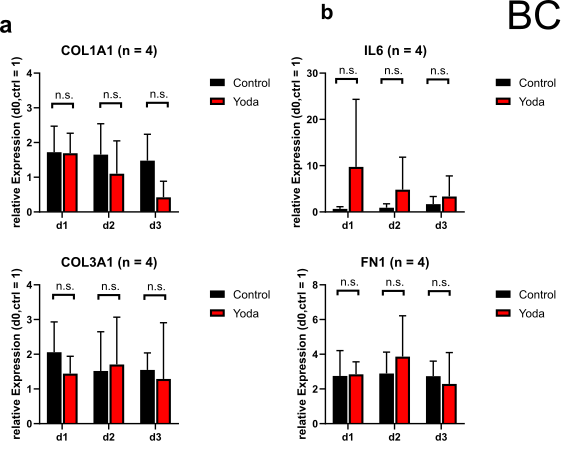
\includegraphics[scale = 0.6]{Collection.png}
    \caption{
    Modest adaptation on transcriptional level as consequence of Piezo1-Activation. \hfill \newline
    \textbf{a}: \colone{}
    \textbf{b}: IL-6
    \textbf{c}: \colthree{}
    \textbf{d}: \textsc{Fn}1. 
    (All Experiments: n = 4). 
    }
    \label{fig:my_label}
\end{figure}


\begin{figure}[htbp]
  \centering
  \includesvg[width=\linewidth]{200205_WesternBlotQuantified_YodaExp_Col1a1.svg}
  \caption{Collagen 1 alpha 1 is reduced }
\end{figure}


\section{\Piezo and osteogenic differentiation}

\begin{figure}[htbp]
  \centering
  \includesvg[width = 0.7\linewidth]{Osteogenic_PCR_Yoda.svg}
  \caption{svg image}
\end{figure}

Something that is reported in literature Here I'm basically going to mention that due to long-term nature of the effect we suspected differentiation. Since Proteins investigated are heavily implicated with Osteogenic differentiation, we looked into osteogenic differentiation. Enter Graph. Even though some tendency can be seen, results of those markers are not significant. 

\section{Reversibility of Piezo1-stimulation}


\begin{figure}
    \centering
    \includesvg{Collective_Long_v1.svg}
    \caption{Tendency of Yoda-effect still visible 7 days after intervention. After 3 days, medium was changed and either supplemented with 10\% FBS (denoted with S+) or serum-free (denoted with S-). (n = 1)}
    \label{fig:my_label}
\end{figure}

In this experiment we wanted to investigate whether the effects seen before would recover after some time and the cells enter a state of pre-intervention homeostasis. One technical issue that we had to solve in this experiment, was the fact that a significant amount of cells showed signs of distress and apoptosis after Yoda1-intervention. In order to allow for sufficient cell survival until we would harvest the cell for analysis, we adapted the protocol from the previous experiment, such that we changed the medium after three days. Half of the cells received serum free MEM\textalpha{}, whereas the other half was administered MEM\textalpha{} with 10\% FBS. 
While we can clearly see that cells proliferate again in reaction to FBS, they don't seem to recover anymore from Piezo1-activation. \myworries{Wrong Text here}

\section{Excursion: Biostability of Yoda1 and Piezo1 mediated apoptosis}
\label{sec:biostability}
We realised that 3 days after the intervention, there was a large decrease in cell count in Yoda1-treated cells when compared to negative control. Next to Piezo1 being implicated in this pro-apoptotic effect, an intrinsic cytotoxicity of Yoda1 could also be an explanation. To test this hypothesis, Uli, in an explorative experiment, exposed both Piezo1-KO and NoT Cell Lines to Yoda1, which showed that the apoptotic effect is dependent on Piezo1 Expression. (Not shown)

\begin{figure}
    \centering
    \includesvg[width = \linewidth]{Yoda_Apoptosis.svg}
    \caption{Light microscopy picture of cells 7 days after intervention both cultured serum-free. Observe the round, \myworries{apoptotic} morphology in the Yoda1-treated samples.}
    \label{fig:yoda_apop}
\end{figure}